\def\mytitle{Boolean Expression to its simplest form using K-map}
\def\mykeywords{}
\def\myauthor{SHAIK KHAJA MASTAN AHMED}
\def\contact{19pa1a04e9@vishnu.edu.in}
\def\mymodule{Future Wireless Communication-(FWC22052)}
\documentclass[10pt, a4paper]{article}
\usepackage[a4paper,outer=1.5cm,inner=1.5cm,top=1.75cm,bottom=1.5cm]{geometry}
\twocolumn
\usepackage{graphicx}
\graphicspath{{./images/}}
\usepackage[colorlinks,linkcolor={black},citecolor={blue!80!black},urlcolor={blue!80!black}]{hyperref}
\usepackage[parfill]{parskip}
\usepackage{lmodern}
\renewcommand*\familydefault{\sfdefault}
\usepackage{watermark}
\usepackage{karnaugh-map}
\usepackage{lipsum}
\usepackage{xcolor}
\usepackage{listings}
\usepackage{float}
\usepackage{titlesec}
\usepackage{amsmath}
\usepackage{algorithm2e}

\titlespacing{\subsection}{0pt}{\parskip}{-3pt}
\titlespacing{\subsubsection}{0pt}{\parskip}{-\parskip}
\titlespacing{\paragraph}{0pt}{\parskip}{\parskip}
\newcommand{\figuremacro}[5]{
    \begin{figure}[#1]
        \centering
        \includegraphics[width=#5\columnwidth]{#2}
        \caption[#3]{\textbf{#3}#4}
        \label{fig:#2}
    \end{figure}
}

\lstset{
frame=single, 
breaklines=true,
columns=fullflexible
}
\thiswatermark{\centering \put(0,-90.0){
\includegraphics[scale=0.05]{IITH logo.jpg}} }
\title{\mytitle}
\author{\myauthor\hspace{1em}\\\contact\\IITH\hspace{0.5em}-\hspace{0.5em}\mymodule}
\date{}
\hypersetup{pdfauthor=\myauthor,pdftitle=\mytitle,pdfkeywords=\mykeywords}
\sloppy
\begin{document}

  \maketitle
\tableofcontents

\section{Introduction}
K maps are used to  Simplify  Boolean Expressions.
The given Expression to solve is
F(S3,S2,S1,S0)=(1,5,6,7,11,12,13,15)

        



\section{karnaugh-map}
        \begin{karnaugh-map}[4][4][1][$S1S0$][$S3S2$]
        \minterms{1,5,6,7,11,12,13,15}
        \maxterms{0,2,3,4,8,9,10,14}
        \implicant{1}{5}
        \implicant{7}{6}
        \implicant{12}{13}
        \implicant{15}{11}
        \end{karnaugh-map}
        Y=S0S1'S3'+S1S2S3'+S1'S2S3+S0S1S3




\section{Components}



\begin{table}[htbp]
 \begin{center}
    \begin{tabular}{|l|c|c|c|c|c|c} \hline \textbf{Component}
  & \textbf{value} & \textbf{quantity} \\
 \hline
Resistor & 220 ohm & 1 \\ \hline
Arduino & UNO & 1 \\ \hline
LED &  & 1 \\ \hline
Bread board &  & 1 \\ \hline
Jumper wires & M-M & 10\\ \hline
\end{tabular}   
\end{center}
\caption{\label{table:dummytable} }
\end{table}


\section{Truth table for given expression}
\begin{table}[htbp]
 \begin{center}
    \begin{tabular}{|l|c|c|c|c|c|c|c|c} \hline \textbf{S3}
  & \textbf{S2} & \textbf{S1} & \textbf{S0}& \textbf{Y} \\
 \hline
        0&0&0&0&0 \\
        \hline
        0&0&0&1&1 \\
        \hline
        0&0&1&0&0 \\
        \hline
        0&0&1&1&0 \\
        \hline
        0&1&0&0&0 \\
        \hline
        0&1&0&1&1 \\
        \hline
        0&1&1&0&1 \\
        \hline
        0&1&1&1&1 \\
        \hline
        1&0&0&0&0 \\
        \hline
        1&0&0&1&0 \\
        \hline
        1&0&1&0&0 \\
        \hline
        1&0&1&1&1 \\
        \hline
        1&1&0&0&1 \\
        \hline
        1&1&0&1&1 \\
        \hline
        1&1&1&0&0 \\
        \hline
        1&1&1&1&1 \\
        \hline
\end{tabular}   
\end{center}
\caption{\label{table:dummytable} }
\end{table}







\section{Connections and results}



Also make connections to arduino UNO ,led and inputs based on table3. 

\begin{table}[htbp]
 \begin{center}
    \begin{tabular}{|l|c|c|c|c|c|c|c|c} \hline \textbf{Arduino UNO}
  & \textbf{5} & \textbf{4} & \textbf{3}& \textbf{2}& \textbf{8}& \textbf{gnd} \\
 \hline
Input&S3&S2&S1&S0&&\\ \hline
led&&&&&+&- \\ \hline
\end{tabular}   
\end{center}
\caption{\label{table:dummytable} }
\end{table}



\begin{table}[htbp]
 \begin{center}
    \begin{tabular}{|l|c|c|c|c|c|c|c|c} \hline \textbf{Sample input}
  & \textbf{S3} & \textbf{S2} & \textbf{S1}& \textbf{S0}& \textbf{LED } \\
 \hline
1&0&0&0&0&OFF\\ \hline
2&0&0&0&1&ON \\ \hline
\end{tabular}   
\end{center}
\caption{\label{table:dummytable} }
\end{table}
\vspace{3mm}
Code Link:
\begin{lstlisting}
https://github.com/19pa1a04e9/FWC-IITH/blob/main/Assignment-1/AVR-GCC/codes/main.c
\end{lstlisting}
\pagebreak

\section{Logic Circuit}
\begin{figure}[!h]
\resizebox {\columnwidth} {!} {
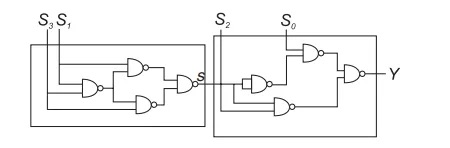
\includegraphics[width=1\columnwidth]{Logic Circuit.jpg}
}
\caption{Logic circuit using four 2-input NAND gates}

\end{figure}



\end{document}